\chapter{Mathematical Modelling and System Identification}
This chapter follows the process of mathematically modelling the quadrotor system. The nomenclature for the kinetics and kinematics has been discussed in Section \ref{SECT_QuadFlightDynamics}. The chapter begins with the dynamic flight model of the craft, focusing on all forces and moments generated by the rotors. The chapter then continues to describe the process of system identification followed to generate the required constants and system parameters for an accurate model. The external disturbances are discussed next, specifically the wind models used in this work. The chapter concludes with an overview of the non-linear simulation generated from the discussion.
	
\section{Dynamic Flight Model}\label{SSECT_DynamicFLightModel}
The dynamic flight model of the craft must cater for all six of the degrees of freedom the craft experiences. The dynamics of this system is modelled as three rotational and three translational degrees of freedom \cite{Moller2015}. To continue deriving the equations of motion, the following assumptions are made: the aircraft is a rigid body, the aircraft has constant mass and $I_{xy}, I_{xz}, I_{yz}$ are all negligibly small.   

The Newton-Euler method of defining the accelerations uses the inertial frame to define the linear accelerations, and the body frame to define the rotational accelerations. Using Newton's first law and the rotation matrix described in \eqref{EQ_RotationMatrix}, the expression for the linear acceleration can be developed and is shown in \eqref{EQ_EulerNewtonInertialMatrix}.

\begin{equation}
\begin{bmatrix} \ddot{N}\\ \ddot{E}\\ \ddot{D} \end{bmatrix} = \begin{bmatrix} 0\\ 0\\ g \end{bmatrix} + \textbf{R} \begin{bmatrix} 0\\ 0\\ \frac{\textbf{T}}{m} \end{bmatrix}
\label{EQ_EulerNewtonInertialMatrix}
\end{equation}

The rotational accelerations of the craft can be similarly described using the moments and the simplified inertia tensor. These rotational rates are described in \eqref{EQ_EulerNewtonRotationMatrix}

\begin{equation}
\begin{bmatrix}\ddot{\phi}\\ \ddot{\theta} \\ \ddot{\psi} \end{bmatrix} = \begin{bmatrix} I_{xx} N  \\ I_{yy} M  \\ I_{zz} L \end{bmatrix}
\label{EQ_EulerNewtonRotationMatrix}
\end{equation}
	
\section{System Identification}
In order to correctly model the system, a thorough system identification needs to be completed. This entails real world measurements of the chosen platform or substantiated evidence from literature for aircraft of similar size and characteristics. The methods and results from these experiments are covered in this section.

	\subsection{Mass and Inertia}
	Using a calibrated scale the mass of the rotorcraft measured at 3.352Kg. 
	
	To calculate moments of inertia, the Bifilar Pendulum method was used. The method is thoroughly described in literature and involves tying the drone from the ceiling allowing it rotate around one axis. Since it is desired to measure the inertias along three axes, three separate test set ups were required. Images of the test set up for a single axis is shown in \ref{IM_BifilarPendulum}. 
	
	\begin{figure}[H]
		\centering
		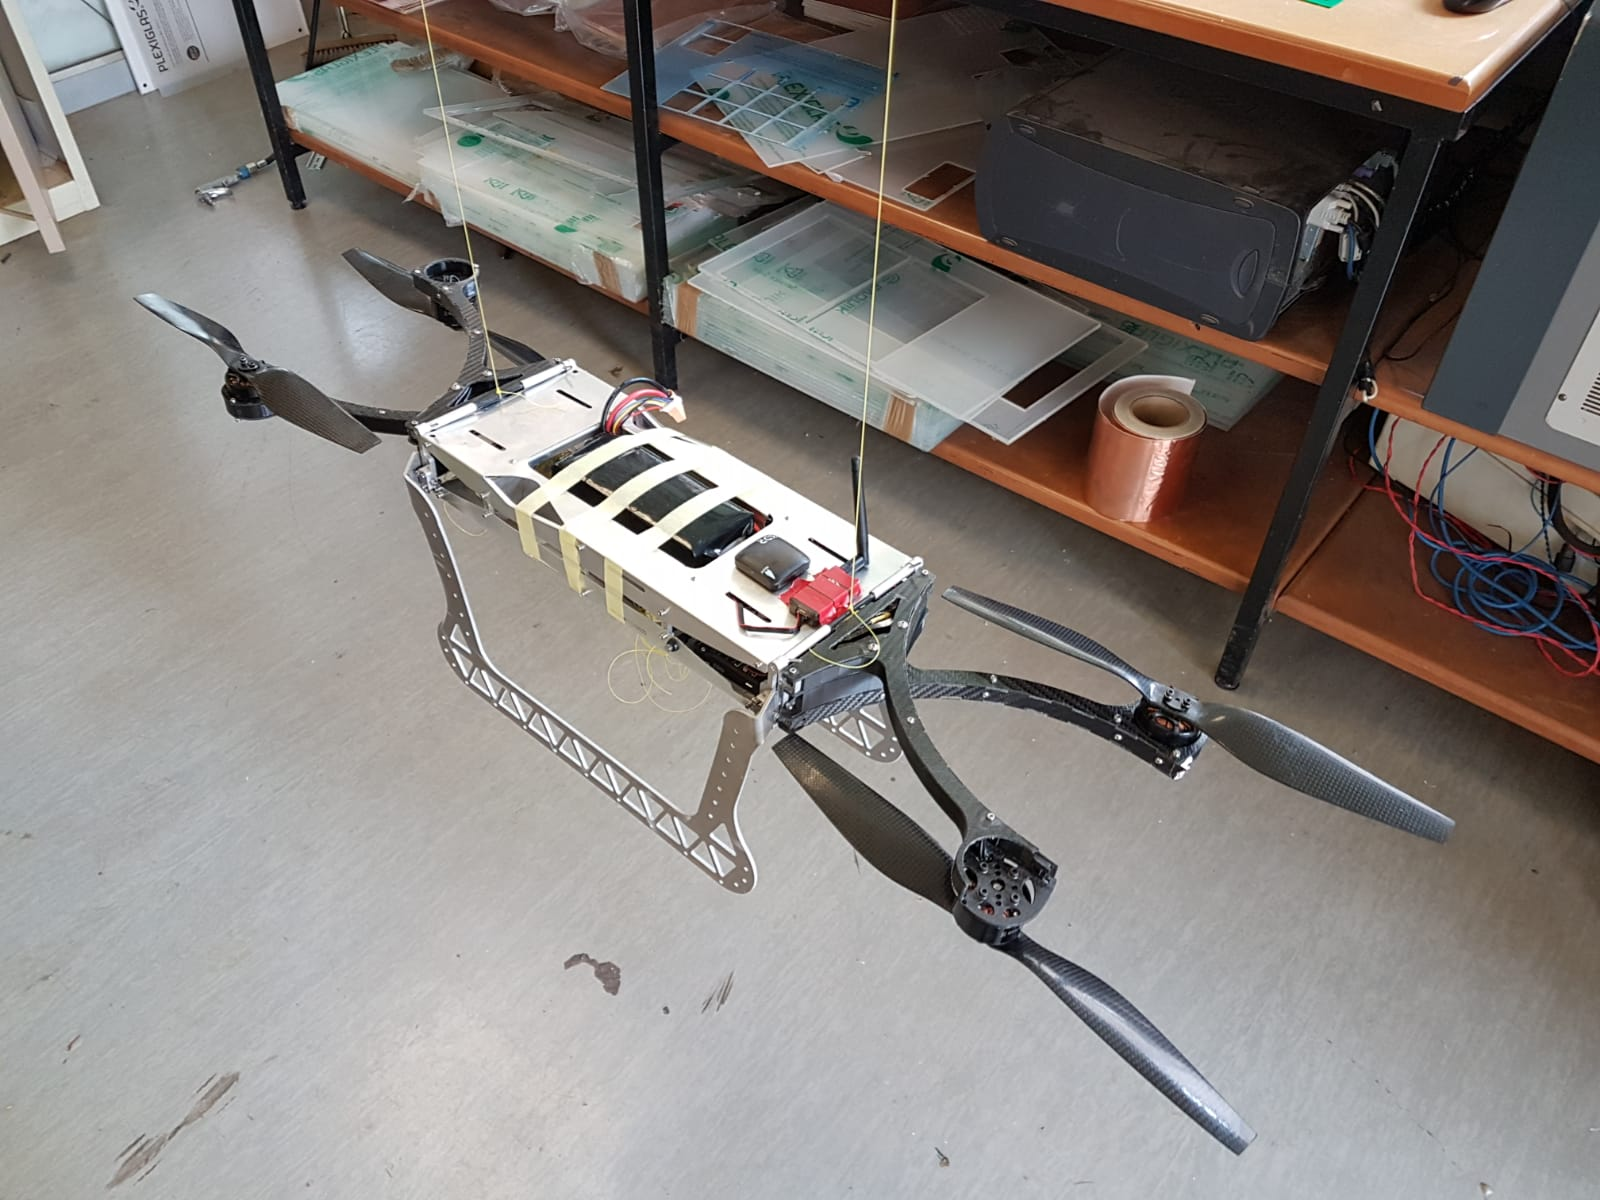
\includegraphics[height = 7.5cm]{Images/BifilarPendulum.jpeg}
		\caption{Bifilar Pendulum for Inertia Measurement}
		\label{IM_BifilarPendulum}
	\end{figure}
	
	Each axis was measured 10 times and the values were averaged out to obtain the final values represented in Table \ref{tab:MomentOfInertia}. To give a representation of measurement variance, the standard deviation is provided along side.
	
	\begin{table}[H]
		\centering
		\begin{tabular}{l | c | c | c |}
			Parameter & Averaged Measured Value & Standard Deviation\\
			\hline\hline
			$I_{xx}$ & 0.025027578 & 0.001063842\\
			$I_{yy}$ & 0.169260024 & 0.000142928\\
			$I_{zz}$ & 0.170196714 & 0.000527406\\
		\end{tabular}
		\label{tab:MomentOfInertia}
		\caption{Measured Moments of Inertia}
	\end{table}
	
	\subsection{Thrust and Moment Profiles}
	In order to correctly validate the thrust characteristics of the drone, each motor rotor pair needed to be evaluated. Each pair was marked and coupled to a load cell. The ESCs were configured to send varying PWMs to the motors. The commands sent to the ESCs and the measured thrust values are plotted together in Figure \ref{IM_ThrustProfiles}. Table \ref{tab:ThrustProfiles} gives the exact maximum and minimum values of each rotor motor pair. 
	
	\begin{figure}[H]
		\centering
		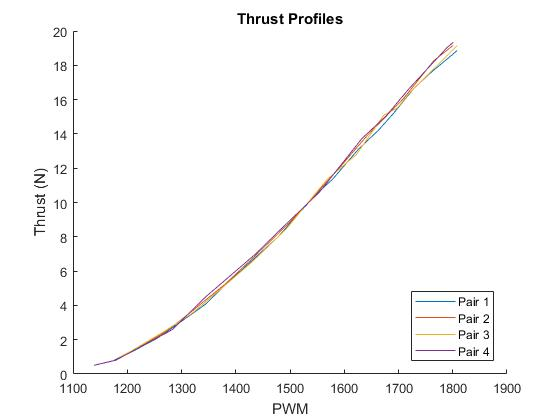
\includegraphics[height = 10cm]{../Design/Mechanical/ThrustProfiles/thrustprofiles.jpg}
		\caption{Thrust Ranges for Motor Rotor Pairs}
		\label{IM_ThrustProfiles}
	\end{figure}
	
	\begin{table}[H]
		\centering
		\begin{tabular}{l | c | c | c |}
			Pair & Max Thrust & Min Thrust\\
			\hline\hline
			$1$ & 18.8558 & 0.7852\\
			$2$ & 19.1489 & 1.1889\\
			$3$ & 19.1434 & 0.9511\\
			$4$ & 19.3369 & 0.5087\\
		\end{tabular}
		\caption{Measured Moments of Inertia}
		\label{tab:ThrustProfiles}
	\end{table}
	
	The motor lag constant for a similar sized craft and rotors was investigated in \cite{Moller2015} and found to be 0.125s. Each rotor is also subject to high frequency noise caused by undesired vibrations. The high frequency noise is modelled as a bandwidth limited white noise applied to each motor separately. 
	
	\subsection{Drag Coefficients}
	The drag coefficients chosen are that typically expected for a flat plate with an effective frontal area, as that seen in the fuselage of the craft. A $C_D$ of $1$ is chosen.
	
	The surface area of the drone was calculated by taking physical measurements of the drone and calculating the surface area from the measurements. Table \ref{tab:DragCoeff} records the calculated surface areas to be used in the calculation of each drag component. The last value in the table is the centre of gravity (COG) which was calculated to be located at the centre of the X and Y axis indicating symmetry along those axes, with a $3.5$\,cm offset in the Z-Axis. The centre of pressure (COP) is assumed as the centre of the craft, creating the required offset for the drag moments described in \ref{SSSECT_Drag}.
	
	\begin{table}[H]
		\centering
		\begin{tabular}{l | c |}
			Parameter & Value\\
			\hline\hline
			$A_x$ & 0.0354\\
			$A_y$ & 0.0693\\
			$A_z$ & 0.4\\
			$C_D$ & 1\\
			$COG$ & [0 0 0.035]\\
			$COP$ & [0 0 0]\\
		\end{tabular}
		\caption{Drag Coefficients}
		\label{tab:DragCoeff}
	\end{table}
	 
	\subsection{Sensor Constants}
	Investigation into the sensors used by the PixHawk, the proposed flight controller module, gives an indication of the sensor accuracy, resolution, noise and speed the drone measurements will be subject to.
	
	The PixHawk uses a combination of gyroscopes, accelerometers and magnetometers. The sensors used for the characterisation are the 6 DOF BMI055 which contains a 3-Axis accelerometer and a gyroscope along with the IST8310, 3-Axis magnetometer. Table \ref{tab:SensorCoeff} lists the extracted data.
	
	\begin{table}[H]
		\centering
		\begin{tabular}{l | c | c | c | c |}
			Sensor & Offset & Resolution & Noise & Maximum Bandwidth\\
			\hline\hline
			Accelerometer & $\pm70$\,mg & $0.98$\,mg & $150$\,$\mu$g/$\sqrt{Hz}$ & $1000$\,HZ\\
			Gyroscope & $\pm1$\,\textdegree/s & $0.1$\,\textdegree/s & $0.014$\,\textdegree/s/$\sqrt{Hz}$ & $1000$\,HZ\\
			Magnetometer & $\pm0.3$\,$\mu$T & $0.3$\,$\mu$T/LSB & NA & $200$\,Hz\\
		\end{tabular}
		\caption{IMU Sensor Coefficients}
		\label{tab:SensorCoeff}
	\end{table}
	
	For location and velocity measurements the GPS sensor used is the Neo-M8N developed by UBlox. Table \ref{tab:GPSCoeff} lists the relevant information obtained from the sensor datasheet.
	
	\begin{table}[H]
		\centering
		\begin{tabular}{l | c | c |}
			Sensor & Accuracy & Maximum Bandwidth\\
			\hline\hline
			Position & $2.5$\,m & $10$\,Hz\\
			Velocity & $0.05$\,m/s & $10$\,Hz\\
		\end{tabular}
		\caption{GPS Coefficients}
		\label{tab:GPSCoeff}
	\end{table}
	
	From the information gathered the sensors can now be modelled accordingly in Simulink. The IMU is modelled using the 3-Axis accelerometer block and the 3-axis gyroscope block in Simulink. The noise is set by using the above documented noise ratios. The GPS model utilises the Band-Limited White Noise Block in Simulink to create appropriate sensor noise. 

	\subsection{Wind Model}
	The wind model is broken into two portions, a constant wind and a more erratic, unpredictable wind both of which flow in the NED frame. The constant wind is defined as a configurable constant in the North East Down frame. The gust component is modelled as shown in Figure \ref{IM_WindModel}. The band limited white noise block is passed through a first order low pass filter to create a more realistic dynamic wind. The gain of the filter can be adjusted to observe effects of larger wind gusts on the craft.
	
	\begin{figure}[H]
		\centering
		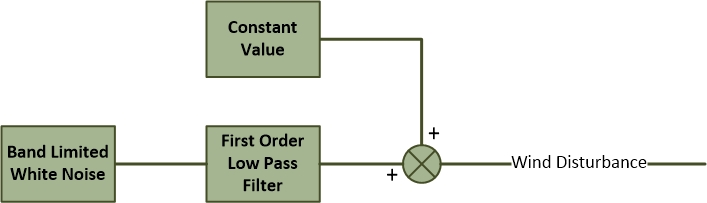
\includegraphics[height = 4cm]{../References/Diagrams/WindModel.jpg}     
		\caption{Wind Model}
		\label{IM_WindModel}
	\end{figure}
	
	The direction is commanded in the NED frame and rotated to apply the applicable forces to the body frame. The direction is modelled with a constant offset and varied by adding a small random number, smoothed by a low pass filter to create a more realistic wind direction variance.
			
\section{Simulation Configuration}\label{SECT_Nonlinear}
This section describes the process of creating the non linear simulation of the aircraft. The drone was modelled in Simulink using a combination of blocks included in the aerospace and control toolboxes, as well as a set of custom blocks. The model is required to successfully predict the position of the craft after being subjected to forces and moments. Using the dynamic flight model created above the bodies linear and rotational accelerations can be calculated by inputting forces and moments into the system. These accelerations can be subsequently integrated to achieve rates and positions. No model is 100\% accurate, however the information recorded in this chapter, when included, should create a solid estimation of the real world craft dynamics.

	\subsection{Motor Mixer}		
	The motor mixer is an important part of the control software running on the onboard computer and thus should be accurately modelled. This portion of code commands the ESCs of the drone to create the desired moments and forces. Section \ref{SSECT_RotorForcesMoments} explains how the rotors have control of four virtual actuators, these are $\delta_Z$, $\delta_{\theta}$, $\delta_{\psi}$ and $\delta_{\phi}$. The motor mixer is responsible for converting these desired moments and forces into actual values of thrust for each rotor.
	
	As Figure \ref{IM_MotorMixer} describes, each motor thrust value is made up of a summation of four thrust values,  $T_Z$, $T_{\theta}$, $T_{\psi}$ and $T_{\phi}$. Each value describes the rotor's contribution to the generation of that specific virtual actuator.
	 
	\begin{figure}[H]
		\centering
		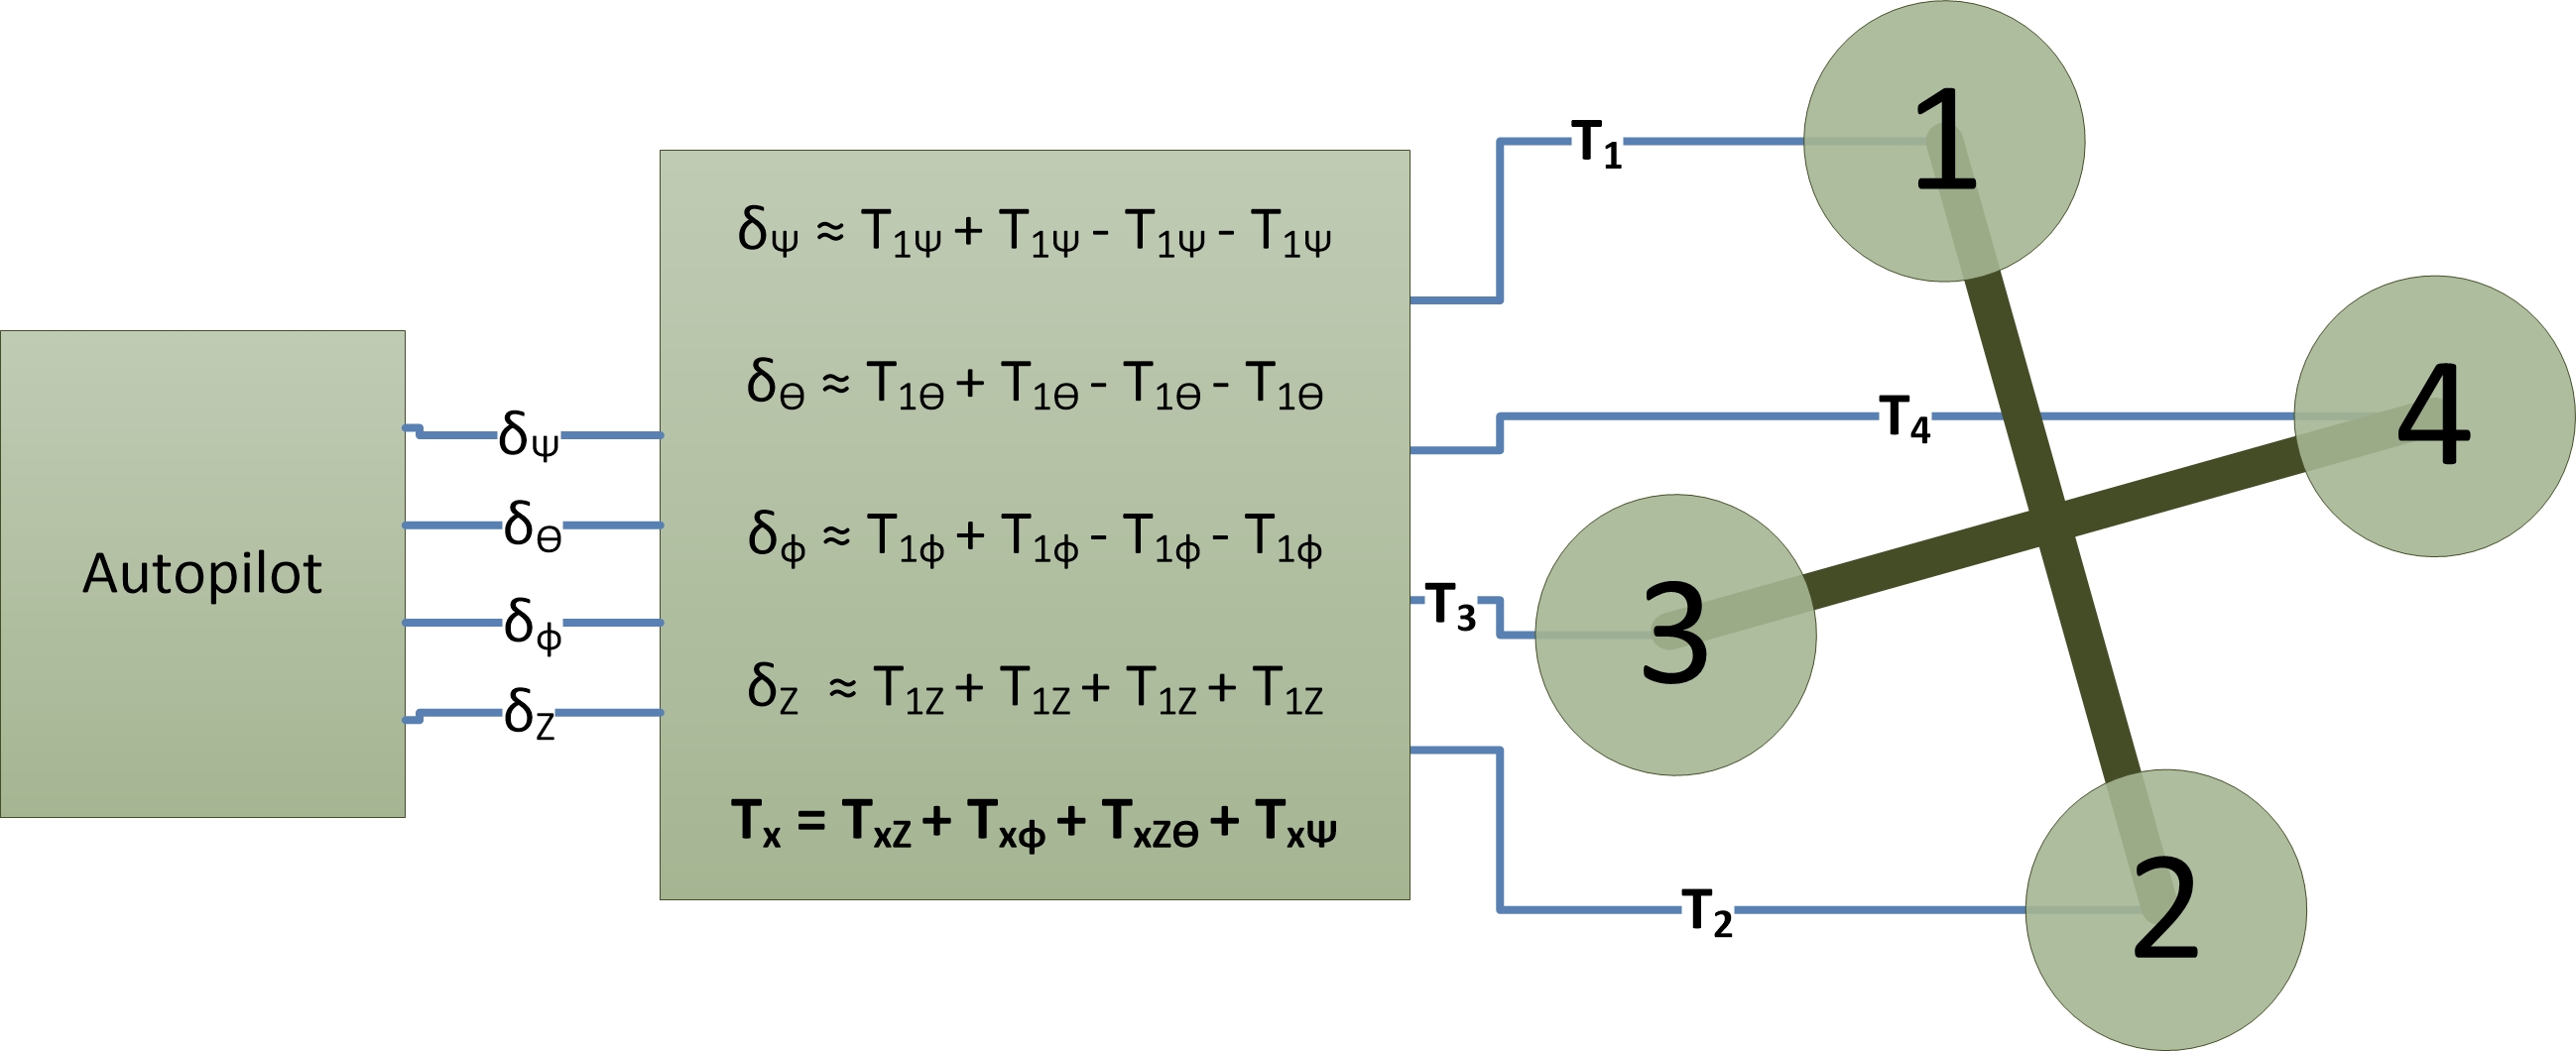
\includegraphics[height = 5cm]{../References/Diagrams/MotorMixer.jpg}
		\caption{Motor Mixer}
		\label{IM_MotorMixer}
	\end{figure}
	
	The motor mixer mathematics is based on the contribution provided by each rotor's thrust to the relevant virtual actuator. Assuming that each rotor only contributes a Z-Force it can be said that each rotor's thrust contributes 100\% of it's power to the virtual actuator $\delta_{Z}$. The roll and pitch virtual actuators are moment contributions and are calculated by evaluating the distance off the centre of gravity. Using the rotor arm length ($l$) and the angle ($\alpha$) a simple trigonometric relationship dictates the roll and pitch contributions. Finally the yaw contribution is calculated by taking into consideration the drag created by each rotor as it generates thrust. This relationship includes the lift to drag ratio ($R_{LD}$) of each rotor and the effective chord length ($r_D$) where the drag force is applied. Using all of these relationships the motor mixer's contribution matrix can be created and is shown in \eqref{EQ_MotorMixerMatrix}. The signs in the matrix are dictated by the body frame notation of positive directions and the placement of the rotors. The yaw contributions are dependant on the rotation direction of the rotors.

	\begin{equation}
	\label{EQ_MotorMixerMatrix}
	Contribution Matrix = 
	\begin{bmatrix}
	-1 & -1 & -1 & -1 \\
	l\sin\alpha & -l\sin\alpha & l\sin\alpha & -l\sin\alpha\\
	-l\cos\alpha & l\cos\alpha & l\cos\alpha & -l\cos\alpha \\
	-\dfrac{r_D}{R_{LD}} & -\dfrac{r_D}{R_{LD}} & \dfrac{r_D}{R_{LD}} & \dfrac{r_D}{R_{LD}} \\
	\end{bmatrix}
	\end{equation}
	
	The values for thrust can subsequently be calculated by multiplying the desired forces and moments by the inverse of the contribution matrix.


		